The Raspberry Pi 3 is a single-board computer that accepts MIPI cameras. This device will be used to connect an infrared MIPI Camera and stream a live video fee from the camera via ethernet. In order to avoid connectivity issues with the Jetson TK-1, the Raspberry Pi 3 has been configured with a static IP address. To assure that the live video fee has a small latency, the Raspberry Pi 3 will be connected to a router. The video feed is being streaming using VLC. 

%%%Change Pictures
\begin{figure}[h!]
	\centering
 	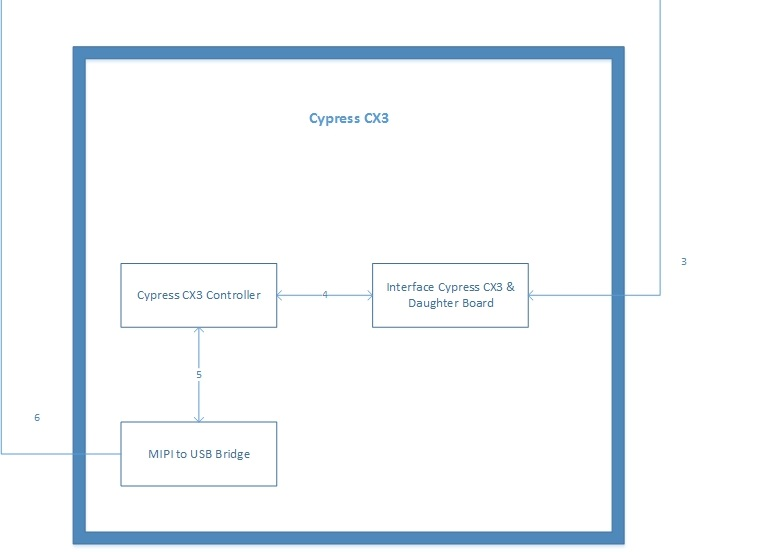
\includegraphics[width=0.60\textwidth]{images/Cypress}
 \caption{Jetson Subsystem Diagram}
\end{figure}


\subsection{Central Processing Unit}
The CPU of the Raspberry Pi is connected to multiple components. One of those components is the camera connector that needs to have a 15 pin ribbon cable in order to accurately receive a video feed from the MIPI camera. In this product, the camera connector is connected to an HDMI Extension Board via a ribbon cable. The CPU of this device also sends the live video fee using VLC via ethernet. All the user needs to have to capture the live video feed is the static IP address of the Raspberry Pi 3. 

%%%Update Imagei
\begin{figure}[h!]
	\centering
 	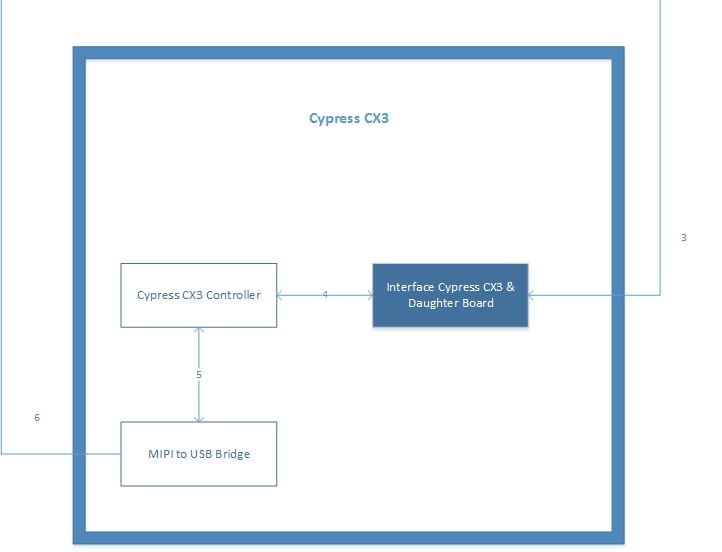
\includegraphics[width=0.60\textwidth]{images/Cypress_Interface}
 \caption{GPID Interface}
\end{figure}

\subsubsection{Assumptions}
The user knows how to connect to the Raspberry Pi 3 via SSH using the Jetson TK-1 terminal.

\subsubsection{Responsibilities}
The responsibility of the Raspberry Pi 3 CPU is to start the live video stream.

\subsubsection{Subsystem Interfaces}

\begin{table}[H]
\caption {Central Processing Unit}
\begin{center}
	\begin{tabular}{ | p{1cm} | p{6cm} | p{3cm} | p{3cm} |}
	\hline
	ID & Description & Inputs & Outputs \\ \hline
	\#03 & HDMI Extension Board & \pbox{3cm}{Input 1 - MIPI Data} & \pbox{3cm}{Output 1 - MIPI Power \\ Output 2 - MIPI Clock} \\ \hline
	\end{tabular}
\end{center}
\end{table}

%%\newline

\subsection{Cypress CX3 Controller}
The main purpose of the CX3 Controller is to interface with the MIPI camera and then transfer the data collected to the CX3 USB interface. The CX3 Controller its also connected to multiple components of the Cypress CX3, but at the moment we have not determined which components will be needed for the Eye Tracker System. For example, we believe that the Eye Tracker System will not need to be connected to JTAG, so those pins on the controller will not be used.

\begin{figure}[h!]
	\centering
 	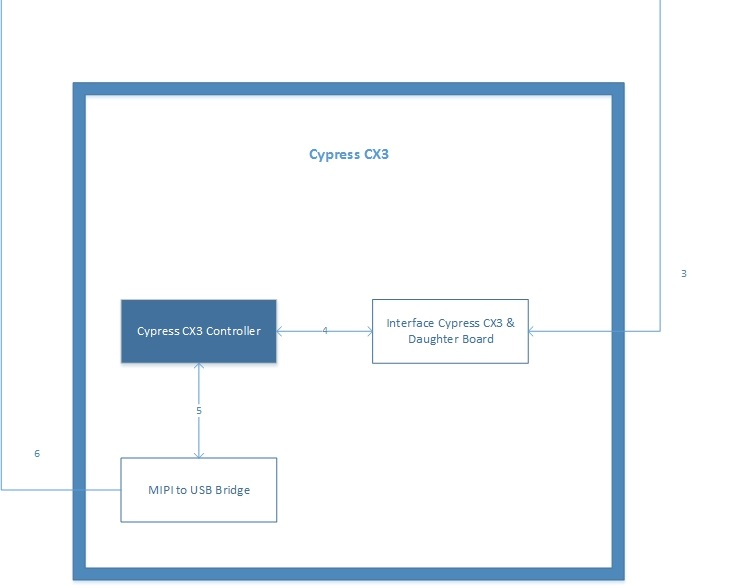
\includegraphics[width=0.60\textwidth]{images/Cypress_Controller}
 \caption{Cypress CX3 Controller interface}
\end{figure}

\subsubsection{Assumptions}
TBD

\subsubsection{Responsibilities}
TBD

\subsubsection{Subsystem Interfaces}
TBD

\begin {table}[H]
\caption {Jetson TK1 Controller Interface}
\begin{center}
    \begin{tabular}{ | p{1cm} | p{6cm} | p{3cm} | p{3cm} |}
    \hline
    ID & Description & Inputs & Outputs \\ \hline
    \#04 & Communication between CX3 Controller and MIPI & \pbox{3cm}{Input 1 - MIPI Data \\ Input 2 - MIPI Clock \\ Input 3 - MIPI Power \\ Input 4 - SDA} & \pbox{3cm}{Output 1 - SCL \\ Output 2 - SDA}  \\ \hline
    \#05 & Communication between CX3 Controller and USB Interface & \pbox{3cm}{Input 1 - SCL \\ Input 2 - SDA} & \pbox{3cm}{Output 1 - MIPI Clock \\ Output 2 - MIPI Data}  \\ \hline
    \end{tabular}
\end{center}
\end{table}
%%\newline

\subsection{MIPI to USB Bridge}
The main purpose of the CX3 USB Interface is to serve as a bridge connection of MIPI camera to USB. The entire system will be powered using the USB connection. This part of the CX3 is also connected to the CX3 Controller and transfers the data collected from the MIPI Camera to a computer via USB. Since this device transfers numerous amounts of data between the CX3 and the MIPI camera, it contains multiple internal clocks.

\begin{figure}[h!]
	\centering
 	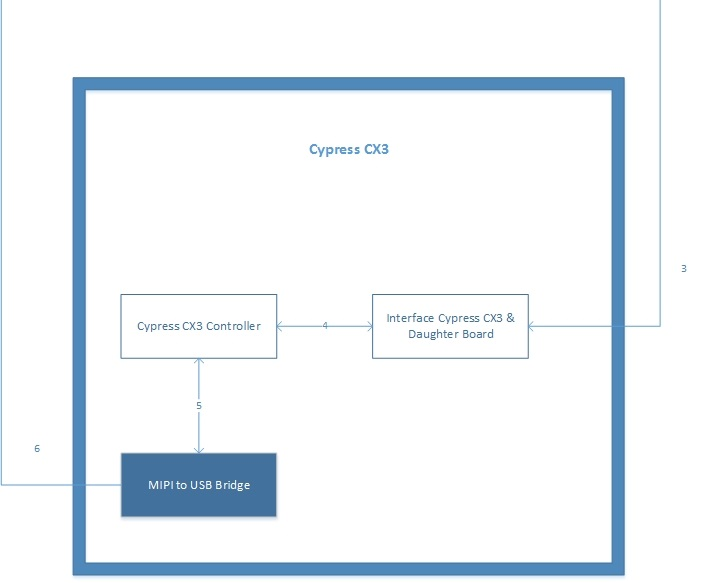
\includegraphics[width=0.60\textwidth]{images/Cypress_MIPI}
 \caption{MIPI to USB Subsystem}
\end{figure}

\subsubsection{Assumptions}
TBD

\subsubsection{Responsibilities}
TBD

\subsubsection{Subsystem Interfaces}
TBD

\begin {table}[H]
\caption {MIPI to USB interface}
\begin{center}
    \begin{tabular}{ | p{1cm} | p{6cm} | p{3cm} | p{3cm} |}
    \hline
    ID & Description & Inputs & Outputs \\ \hline
    \#05 & Communication between USB Interface and CX3 Controller & \pbox{3cm}{Input 1 - MIPI Clock \\ Input 2 - MIPI Data \\ Input 3 - CX3_GPIO} & \pbox{3cm}{Output 1 - SDA \\ Output 2 - SCL}  \\ \hline
    \#06 & Communication between USB Interface and Computer & \pbox{3cm}{N/A} & \pbox{3cm}{Output 1 - USB Data}  \\ \hline
    \end{tabular}
\end{center}
\end{table}
